\section{Задание 1. Интеграл функции одной переменной}

\textbf{Условие.}

В задачах проведите исследование:

1.Составьте математическую модель задачи: введите обозначения, выпишите данные,  составьте уравнение (систему уравнений), содержащее неизвестное.

2.Решите задачу аналитически.

3.Сделайте графическую иллюстрацию к решению задачи.

4.Запишите ответ.

\vspace{5mm}

\begin{multicols}{2}
    Вычислите силу давления воды на пластинку,
    вертикально погруженную в воду,
    считая, что удельный вес воды равен 9,81 кН/м$^3$.
    Результат округлите до целого числа.
    Форма, размеры и расположение пластины указаны на рисунке.

    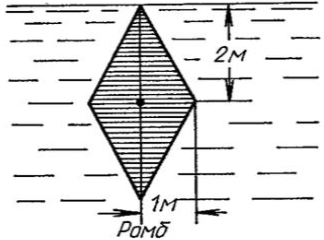
\includegraphics[width=5cm]{images/1a1}

\end{multicols}

\vspace{10mm}

\textbf{Решение.}

It is empty but you can fill it!

\textit{Ответ}: It is empty but you can fill it!
\clearpage
